\documentclass[fleqn,letterpaper,12pt]{article}
\usepackage[utf8]{inputenc}
\usepackage{amsmath, amssymb}
\usepackage{graphicx}
\usepackage{hyperref}
\usepackage{times}
\usepackage{ulem} % Para subrayado
\usepackage[T1]{fontenc} % Para mejorar la compatibilidad de fuentes
\usepackage{lmodern} % Para evitar problemas con la fuente Times
\usepackage{parskip} % Elimina la sangría y añade espaciado entre párrafos
\usepackage{changepage}
\usepackage{amsmath}
\usepackage{ragged2e}
\usepackage[top=2.54cm, bottom=2.54cm, left=2.54cm, right=2.54cm]{geometry} % Reduce los márgenes

\title{}
\author{}
\date{}

\begin{document}

\begin{titlepage}
    \centering
    
\includegraphics[width=0.95\textwidth]{tecnologico-de-monterrey-blue.png} % Reemplaza con la ruta del logo
    \vspace{1cm}

    {\textbf{Instituto Tecnológico y de Estudios Superiores de Monterrey}\par}
    {\textbf{Campus Guadalajara}\par}
    \vspace{1cm}

    {\textbf{Fundamentación de la robótica}\par}
    {\large Gpo 101\par}
    \vspace{1cm}

    {\textbf{Ensayo}\par}
    {\large Control de posición pd=g(Q)\par}
    \vspace{1cm}

    {\textbf{Presenta}\par}
    Sofia Arias Villa \hspace{3cm} A01642380
    \vspace{1cm}

    {\textbf{Profesores}\par}
    Eduardo Francisco Sánchez Ocampo
    \vspace{1cm}

    {\textbf{Fecha de entrega}\par}
    16 de marzo de 2024

\end{titlepage}

\textbf{Función de Lyapunov y Estabilidad}

La función de Lyapunov es una herramienta matemática utilizada en el análisis de la estabilidad de sistemas dinámicos, especialmente en sistemas no lineales. Permite determinar si un punto de equilibrio de un sistema es estable, asintóticamente estable o inestable sin necesidad de resolver explícitamente las ecuaciones diferenciales del sistema.

De la teoría clásica de la Mecánica, es sabido que un sistema es estable si su energía, una función positiva, es continuamente decreciente hasta alcanzar el estado de equilibrio \cite{ogata1990modern}. El segundo método de Lyapunov es una generalización de este hecho. Lyapunov demostró que ciertas otras funciones aparte de la función energía pueden ser usadas para la determinacioón de la estabilidad del punto de equilibrio de un sistema.

Los sistemas no lineales son más complejos y pueden mostrar comportamientos que los lineales no tienen. Por ejemplo, mientras un sistema lineal solo tiene un punto de equilibrio (un estado en el que el sistema se mantiene si no hay perturbaciones), un sistema no lineal puede tener varios. Además, en los sistemas lineales, si el punto de equilibrio es estable, el sistema siempre convergerá a él sin importar cómo empiece. En cambio, en los sistemas no lineales, hacia cuál equilibrio converge el sistema depende de su estado inicial. La estabilidad es una de las propiedades más importantes en los sistemas dinámicos, pero analizarla puede ser más o menos complicada dependiendo del tipo de sistema.

Las condiciones de Lyapunov son un conjunto de requisitos que debe cumplir una función $V(x)$ para garantizar la estabilidad de un punto de equilibrio en un sistema dinámico. 

\begin{adjustwidth}{1.25cm}{0cm}
    La función $V(x)$ debe ser definida positiva en una región alrededor del punto de equilibrio:

    \begin{adjustwidth}{1.25cm}{0cm}
    $V(x) > 0$ para todo $x \neq 0$, y $V(0) = 0$.
    \end{adjustwidth}
\end{adjustwidth}

\begin{adjustwidth}{1.25cm}{0cm}
    La derivada de $V(x)$ con respecto al tiempo debe ser definida negativa en la misma región:
\end{adjustwidth}

\vspace{-9mm} % Reduce el espacio entre estos dos bloques

\begin{flalign*}
    & \hspace{1.4cm} \dot{V}(x) = \nabla V \cdot f(x) < 0 \quad \text{para todo } x \neq 0.
\end{flalign*}

La desventaja de este método es que no hay un método sistemático para hallar una función de Lyapunov por lo tanto hay que proponer una función candidata a función de Lyapunov y probar si la misma cumple con los requisitos de estabilidad.

\vspace{9mm}

\uline{Estabilidad según Lyapunov}

\vspace{4mm}

\raggedright
\begin{tabular}{l p{12cm}} % Primera columna alineada a la izquierda, segunda con ancho fijo
    Estabilidad & El sistema no diverge del equilibrio, pero tampoco converge a él; simplemente se mantiene cerca. \\
    Estabilidad asintótica & El sistema no solo se mantiene cerca del equilibrio, sino que también converge a él con el tiempo. \\
    Inestabilidad & El sistema diverge del equilibrio, incluso si inicialmente estaba cerca. \\
\end{tabular}
\justifying

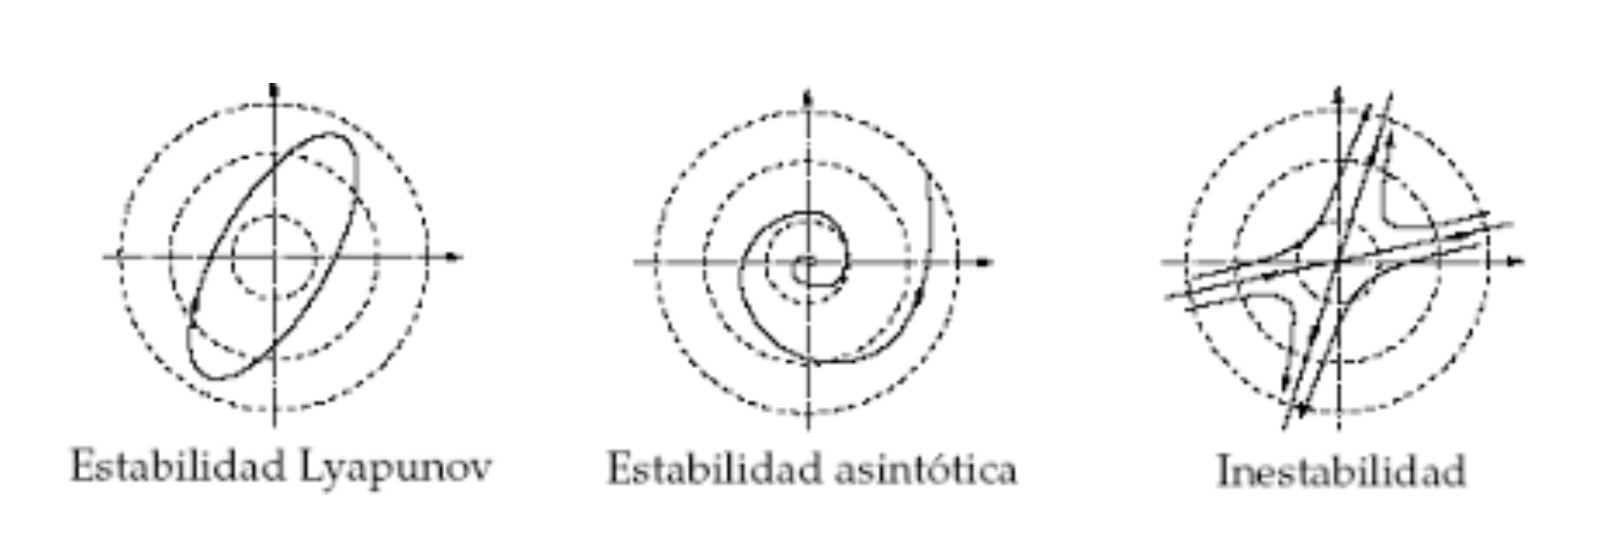
\includegraphics[width=0.75\textwidth]{inestabilidades.jpeg}

\textbf{Controlador PID}

El control PID (Proporcional, Integral, Derivativo) es el método de control más usado en la industria y es ampliamente aceptado en todo el mundo. El control PID combina tres acciones básicas: proporcional, integral y derivativa. Estas acciones se ajustan para obtener el mejor rendimiento del sistema.

\vspace{1mm}

\raggedright
\begin{tabular}{l p{11.6cm}} % Primera columna alineada a la izquierda, segunda con ancho fijo
    \uline{Respuesta proporcional} & Determina la relación entre la respuesta de salida y la señal de error. En general, aumentar la ganancia proporcional aumentará la velocidad de respuesta del sistema de control. \\
    \uline{Respuesta integral} & El componente integral suma el término de error en el transcurso del tiempo.  \\
    \uline{Respuesta derivativa} & El componente derivado hace que la salida disminuya si la variable del proceso aumenta rápidamente. La respuesta derivada es proporcional a la tasa de cambio de la variable del proceso.  \\
\end{tabular}
\justifying

El control PID opera dentro de un sistema de ciclo cerrado, un mecanismo que utiliza sensores para medir la variable de proceso (como temperatura, presión o flujo) y proporcionar retroalimentación constante. Esta información se compara con el punto de referencia (el valor deseado), y la diferencia, conocida como error, es procesada por el algoritmo de control (compensador) para determinar la salida del actuador. El sistema debe manejar perturbaciones, que son señales externas (como una corriente de aire frío) que afectan la variable de proceso.

\vspace{1mm}

\textbf{Función propuesta}

El sistema que estamos analizando es un péndulo simple considerando la fricción cuya dinámica está dada por la siguiente ecuación:

\vspace{-7mm}

\begin{flalign*}
    & \hspace{5cm} mL^2 \ddot{q} + b \dot{q} + mgL \sin q = \tau,
\end{flalign*}

\begin{tabbing}
    $\theta$ \hspace{1cm} \= ángulo del péndulo \\ 
    $m$ \> Masa del péndulo \\ 
    $L$ \> longitud del péndulo \\ 
    $b$ \> coeficiente de fricción \\ 
    $g$ \> aceleración debido a la gravedad \\ 
    $\tau$ \> torque de entrada aplicada al péndulo 
\end{tabbing}
Por simplificación vamos a igualar m=1, L=1, b=0.1 y 9.8=9.81.

Definimos las variables de estado:
\vspace{-3mm}
\[
x_1 = q
\]
\vspace{-3mm}
\[
x_2 = \dot{q}
\]
\vspace{-3mm}
\[
\dot{x}_1 = x_2
\]
\vspace{-3mm}
\[
e = \Theta_d - x_1
\]
\vspace{-3mm}
\[
\dot{e} = -x_2
\]

La dinámica del sistema se puede reescribir en forma de espacio de estado:

\vspace{-7mm}

\begin{flalign*}
    & \hspace{5cm} \dot{x}_2 = -9.81 \sin(x_1) - 0.1 x_2 + \tau
\end{flalign*}

Proponemos un controlador:

\vspace{-7mm}

\begin{flalign*}
    & \hspace{5cm} \tau = -kp x_1 - kd x_2 + G(x_1)
\end{flalign*}

\hspace{1.25cm} $kp$ y $kd$ son las ganancias del controlador.

\hspace{1.25cm} $G(x_1)$ es un término de compensación para eliminar la gravedad:

\vspace{-7mm}

\begin{flalign*}
    & \hspace{5cm} G(x_1) = -9.81 \sin(x_1)
\end{flalign*}

Sustituyendo el controlador en la dinámica del sistema:

\vspace{-7mm}

\begin{flalign*}
    & \hspace{2cm} \dot{x}_2 = -9.81 \sin(x_1) - 0.1 x_2 + \left( -kp x_1 - kd x_2 + 9.81 \sin(x_1) \right)
\end{flalign*}

Simplificando obtenemos:

\vspace{-9mm}

\begin{flalign*}
    & \hspace{5cm} \dot{x}_2 = -kp x_1 - (kd + 0.1)x_2
\end{flalign*}

En forma matricial esto se puede escribir como:
\[
\begin{bmatrix} \dot{e} \\ \dot{x}_1 \\ \dot{x}_2 \end{bmatrix} = 
\begin{bmatrix} 0 & 0 & -1 \\ 0 & 0 & 1 \\ -K_p & 0 & -(K_d + 0.1) \end{bmatrix}
\begin{bmatrix} e \\ x_1 \\ x_2 \end{bmatrix}
\]

\uline{Función de lyapunov propuesta}

\vspace{-9mm}

\begin{flalign*}
    & \hspace{5cm} V(x) = a \left( 1 - \cos x_1 \right) + \frac{1}{2} x_2^2
\end{flalign*}

Análisis de \( V(x) \):

\( (1 - \cos x_1) \) es siempre no negativa y es 0 solo cuando \( x_1 = 2\pi n \), donde \( n \) es un entero.

\( \frac{1}{2}x_2^2 \) es siempre positiva gracias al exponente cuadrado y es 0 solo cuando \( x_2 = 0 \).

\textbf{por lo tanto \( V(x) \) es definida positiva}

Análisis de \( V(x) \):

La derivada de la función \( \dot{V}(x) = a(1 - \cos(x_1)) + \frac{1}{2}x_2^2 \) es:

\vspace{-9mm}

\begin{flalign*}
    & \hspace{2cm} \dot{V}(x) = a x_2 \sin(x_1) - a x_2 \sin(x_1) - b x_2^2
\end{flalign*}

\textbf{Bibliografía}
\begin{thebibliography}{9}
    \bibitem{ogata1990modern} K. Ogata, \emph{Modern Control Engineering}. Prentice Hall, 1990.
    \bibitem{ni_pid} Explicaci\'on sobre el controlador PID y la teor\'ia. NI, 2006. Disponible en: \url{https://www.ni.com/es/shop/labview/pid-theory-explained.html}
    \bibitem{wu2018adaptive} Q. Wu, \emph{Adaptive Sliding Mode Neural Network Control for Nonlinear Systems}. Elsevier, 2018. Disponible en: \url{https://www.sciencedirect.com/book/9780128153727/adaptive-sliding-mode-neural-network-control-for-nonlinear-systems}
\end{thebibliography}

\end{document}
